\section{Discussion}\label{sec:discussion}

%Discuss the results. What is the outcome of your experimetns?
This section shortly discusses the empirical results and then extensively compares the findings of this work to the existing literature while trying to explain some of the differences. It is concluded by a subsection describing the limitations and possible extensions of this work. 

\subsection{Our work}
This subsection discusses our findings. First it will analyze the possible reasons behind the influence of input shuffling to the learning rate. Second it will conclude with the discussion of unexpected results. 

\subsubsection{Shuffling and learning rate with SGD}
In this subsubsection we will use the term advanced optimzers for Adagrad and Adam. The models was able to use a higher learning rates when SGD was combined with input shuffling in comparison to as when not. Therefore, arises the questions why these phenomena happen, especially as it did not happen with advanced optimizers.  \\
First, we suspect our batched version of the Skip-Gram model with negative sampling (SGNS), to be at the origin of this phenomena. In consequence to this batched version, when input shuffling is not used a lot of words will appear multiple times in the same batch, as explained in Section \ref{ssec:shuffling}. Therefore, the gradients will be an average of all the training samples. When the input is shuffled, less words will appear multiple time which will make the gradients more precise.\\
Second, advanced optimizers have a way to counter-attack this issue, namely adaptive learning rates, explained in Section \ref{ssec:results_adagrad}. Adaptive learning rates counter attack the issue in the following way: high frequency words  will appear more often multiple times in a batch, they will also have lower learning rates. Therefore the impact of appearing in the same batch will be reduced. \\  The two above arguments could explain why a higher learning rate combined with SGD achieved better results with input shuffling but not when advanced optimizers are used. 

\iffalse
\subsubsection{Large differences with NAG and SGD when using shuffling}
SGD and NAG both have very different values when using shuffling in comparison to unshuffled input, as shown in figures \ref{fig:results_sgd} and \ref{fig:results_nag}. We do not only attribute those results to input shuffling but partially also to a good random initialization guess. Due to a lack of time these experiments were not replicate more than once.
\fi 

\subsection{Comparison to Gensim}
This subsection will compare our finding extensively to Gensim \citep{gensim}. As explained in Section \ref{ssec:gensim}, Gensim is optimized to have a very high throughput, this made it possible to achieve a lot of computations. Furthermore, Gensim provides access to the loss and the resulting word embeddings, which facilitated the comparison process.
This subsection is structured as follows: first it will describe the used configuration of Gensim, second it will compare Gensim to our implementation of the SGNS with the use of SGD and finally compare our model with Adam to Gensim. A graphic showing the comparison of our models to Gensim can be found in Figure \ref{fig:gensim_vs_adam}.


\subsubsection{Configuration of Gensim}
To compare our-self in a correct  manner we used the same dataset, with the same preprocessing parameters, i.e subsampling and min count. The hyper parameters of the network (window size, embedding size, number of negative sample, exponent to which the unigram distribution, which decides how a negative sample is used, is raised) are equivalent to our parameters described in Section \ref{ssec:config}. The only difference with our model is the learning rate. Gensim has a starting learning rate of $0.025$ and linearly decrease it at every epoch to $0.0001$.

\subsubsection{Gensim vs. SGD}
As stated earlier, we are not going to compare this work to Gensim in run time. Gensim is heavily optimized and written in cython\footnote{https://rare-technologies.com/word2vec-in-python-part-two-optimizing/}, which is 23x faster than plain Numpy. Since we used PyTorch the difference is not that big, but still remains. As shown in Figure \ref{fig:gensim_vs_adam} the convergence time was not the same between our implementation and Gensim. There are different possible reasons why this could be the case:\\ First, our batched approach could hinder performance in terms of convergence time since our loss function is not exactly the same. We compute the loss for multiple training samples by taking the sum over each score which is individually used as a loss by Gensim.\\ Finally, another possibility is the decay of the learning rate used by Gensim. In fact, decaying the learning rate has been proven in a lot of work to decrease the convergence time. Gensim linearly decreases the learning rate, as we did not use this technique, the decay of the learning rate could help explain the noted differences. \\ The first hypothesis, the fact that we used a batched approach, may be confirmed by the fact that when combined with input shuffling SGD does perform closer to Gensim, going from 7 to 5 epochs to converge, as input shuffling reduces the number of co-occurrence of the same word in a batch.
Know the question arises if the 3 epochs, that Gensim is better can be explained by the batched approach and the learning rate decay.

\subsubsection{Gensim vs. Adam}
The Adam optimizer did outperform the Gensim application in quality of word embeddings (only slightly: 0.01 correlation coefficient better) and convergence time. Adam converged in 2 epochs while Gensim in 4. To confirm the achieved results we ran each computation 40 times. The results can be seen in Figure \ref{fig:gensim_vs_adam}.

\begin{figure}[h]
\centering
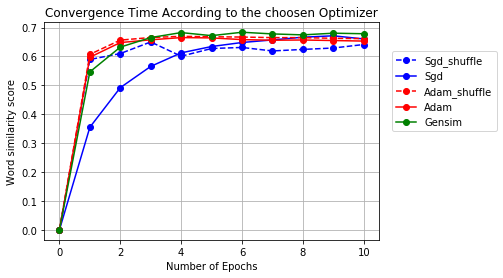
\includegraphics[scale=0.3]{images/comparison}
\caption{Convergence time of SGD and Adam compared to Gensim}
\label{fig:gensim_vs_adam}
\end{figure}

\subsection{Future Work}
This work shows that the convergence time of the SGNS could be improved by using input shuffling and advanced optimizers. As with every work, there still exists possible extensions. First and foremost an aspect of our implementation that can be prejudicial is that we only extensively tested our model with one small dataset. The fact that we only used one dataset as well that it's a small one is problematic. \\ 
~~\textit{Problem with a small dataset:} \\ By using a very small dataset we do not use the model in the condition it is most needed for, as the dataset used in practice usually consists of more than 1 billion words. There is a small argument that can be made for machine translation as the use of small parallel corpus is not unusual in this field. \\
~~\textit{Problem with using only one dataset:}\\
It has been shown that some optimizers perform better with specific shapes of loss functions. To make a compelling argument it's necessary to show that our model with the use of input shuffling and Adam as its optimizer also outperforms Gensim with other data sets.\\
Finally, as it wasn't the goal of our implementation to outperform Gensim in run time, one could improve an already existing, optimized version, with input shuffling and advanced optimizers and should achieve a better run time than Gensim.